\documentclass[a4paper,fleqn]{cas-dc}
\usepackage[numbers]{natbib}
\usepackage{kvoptions,ltxcmds,refcount,hyperref}
\usepackage{amsmath,amsthm,amssymb,braket, graphicx, appendix, empheq, subfig, float, geometry}
\begin{document}
\shortauthors{DCC-RGV}
\title[mode = title]{Testing MD Simulations of Amorphous Carbon.}
\author[1]{Daniel Castillo-Castro}[type=editor]
\author[1]{Rafael González-Valdés}[type=editor]
\address[1]{Centro de Óptica e Información Cuántica, Universidad Mayor, Camino la Pirámide 5750, Huechuraba, Santiago de Chile.}
\begin{abstract}
Amorphous Carbon (aC) is a material of recent interest in Material Sciences. For all its applications is of fundamental importance the evaluation of mechanical and thermodynamical properties. In this paper an Classical MD simulation study is presented and compared with different interatomic potentials. This study was done using several empirical potentials, putting de aC samples made from simple cubic lattices into temperature ramps. For all samples it was measured phase change point to graphite and bulk modulus, looking for thermodynamical properties of the material. It was obtained phase change temperatures of the order of $2000 K$ for different potentials and Bulk modulus of the order of $200-300 GPa$. The best achievement of all potential was reached by EDIP potential.
\end{abstract}
\begin{highlights}
\item 
\item 
\item 
\end{highlights}
\begin{keywords}
Amorophous Carbon\\ Elastic Properties \\Classical Dynamics
\end{keywords}
\begin{graphicalabstract}
\end{graphicalabstract}
\maketitle
\section{Introduction}
In last years, one of the most researched topics in the field of Quantum Information is Diamond NV Color Centers, que came from a point defecto in diamond of 3m symmetry, changing 2 carbon atoms to 1 nitrogen atom and a valence in direction $<111>$.\cite{NVDiamond} Into this area, a recent research interest is nanodiamonds NV center realisation. This nanodiamonds can be considered as tiny sections into an aC bulk with diamond chemical structure (sp$^3$ bond type majority, if it has an sp$^2$ bond type majority, the section is a nanographite). All this makes aC a very interesting material for theoretical and experimental Quantum Optics and Quantum information scientists.

Beyond this, thermodynamics analysis for a bulk material is of fundamental interest. It was demonstrated a relationship between Quantum Information and Quantum Thermodynamics. First of all, because both theories share the concept of Entropy, and this suggest links between the both ones \cite{QTh}. This fact brought studies realisation about information flux and their thermodynamic effects, for example, to spin systems. \cite{ThermoQIFlow} Because all this thermodinamic aC properties analysis results a great interest research area, by the algorithm used to obtain this properties can be undestood as informatical processes as an analogy, similar as it can be seen in some references. Considering some carbon allotropes as limit cases and using numerical method by a similar way of simulations of another materials.  \cite{ThermoFlow}. 
\section{Method}
For the code needed to obtain the properties, it will be used  Classical Molecular Dynamics, that allows to calculate vibrational spectra, linking it with experimental results. The computational results must be read carefully and it will be recommendable to compare them with results made with more sophisticated methods as, for example DFT. By the way, for analysis made in this work, Classical Molecular Dynamics simulation will be of great interest. 

Considering the last paragraph, Marks\cite{ACPot1} purposes a method for making aC samples from a cubic arrange of carbon atoms, whose interatomic distance can variate final AC bulk percentage of sp$^3$ bonds (this indicates the bulk zones that behaves like diamond). While initial interatomic distance is less (equivalent to say that the initial density is greater), it will be a greater bond sp$^3$ percentage after the process (this means that all the aC bulk is diamond-like). The method consists in a sample quenching from $300K$ to $10000 K$ in $0.25 ps$ and a slow annealing process of $5ps$. After this, to make thermodynamical properites measurements, a very slow simulation in NPT of $25 ps$ was made. It has to be considered that system variables, like temperature and pressure, can be calculated in Classical Molecular Dynamics as time averages of  properties of atoms in the system. So, for more precision in properties results is recommendable to take the average in a way that could be representative of systems that start in thermal equilibrium. A simple process scheme can be seen in Figure~\ref{fig:carbon}.

As it was mentioned before, chosen potential to measure will be always an approximation to the real system. So, for interest systems some approximations are more accurate that another ones. Marks' team has developed EDIP potential, that has a very good accuracy for carbon allotropes samples (aC included) according to studies that compares its achievement with potentials like REBO or COMB for creation and destruction of chemical bonds \cite{ACPot2}. A similar procedure will be use to measure properties like phase changes related with temperature y Bulk Moduli, topics of great importants because all the written before in this report.

    \begin{figure}
        \centering
        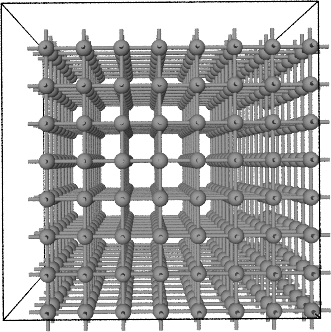
\includegraphics[width=0.15\textwidth]{carbon1.png}
        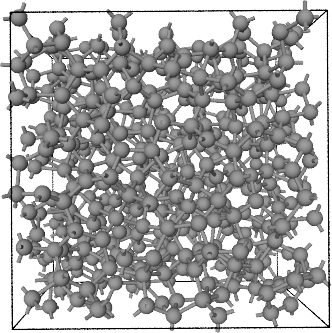
\includegraphics[width=0.15\textwidth]{carbon2.png}
    \caption{The Used Process takes a cubic arrange of carbon atoms (above) and transform it to aC samples (below) with bonds sp$^3$ percentages that has to be defined.To every potential and initial interatomic distance a different sp$^3$ percentage will be obtained. }
    \label{fig:carbon}
   \end{figure}

\section{Results and Analysis}
\subsection{Phase changes}
 In Figure~\ref{fig:meltproc} it is show a sample quenching. The work initial objective was to find melting point values for aC, but it was observed a structural phase change to structural graphite y instead a change of phase from solid to liquid as expected. This agrees with carbon phases derivation made in LHC, that predicts this phase change in a high temperature ($2000- 3000K$) y atmospheric pressure.\cite{Zazula}  
 \begin{figure}
    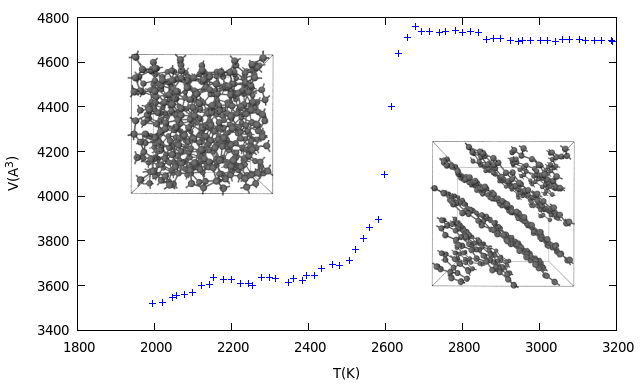
\includegraphics[width=0.5\textwidth]{melting.png}
    \caption{Phase change process from aC to graphite it is shown here. Sample is at atmospherical pressure and is driven into a fast and a slow temperature ramps. It was plotted the results average in the both ramps.}
      \label{fig:meltproc}
\end{figure}
 Beyond this, it will be shown in this report phase change points (for the mentioned phase change) y Bulk Moduli for aC systems. Bulk Moduli are defined as material compression resistance and it was theoretically defined as:
 \begin{equation} K=-v\frac{dP}{dV}, \end{equation} Where V is the volume and P the pressure. 
 
 Work was done with potentials used in \cite{ACPot1} like REBO , BOP , COMB , ReaxFF and Tersoff, including EDIP as a reference, even if the chosen potentials was the ones that gives better results and used a suitable computing time. It was needes, trying to following the aC making secuence, to do phase change point and Bulk Modulus calculus with the same potential used in the process explained before. For any sample is was measured, sp$_3$ bond percentages, using the program OVITO  \cite{Ovito}, taking  final samples and calculating bonds between all atoms, considering atoms at distance less than $2$\AA \space like tangled atoms. 

Phase change points measurements for all samples it was obtained looking dynamics inside the sample by OVITO, these observations were compared with plots that indicate phase change process produced by a quick volume grow in a short temperature interval lesser than $200K$. In Figure~\ref{fig:meltdata} this process was plotted. It was tested for  AIREBO (Adaptativa Intermolecular REBO), BOP, EDIP, ReaxFF y REBO potentials. 

In Figure~4 a phase change temperature values decrease related with a sp$^3$ bond percentage increase was observed. This result can be explained considering that while the sample is more diamond-like the phase change starts at a lower temperature, that agrees with phase diagram shown in Zazula article ~\cite{Zazula}, that indicates than at atmospherical pressure aC-graphite transition was ocurred. Unstable defects with sp$^1$ type bonds that desappears at temperature changes were observed too.
    \begin{figure}
        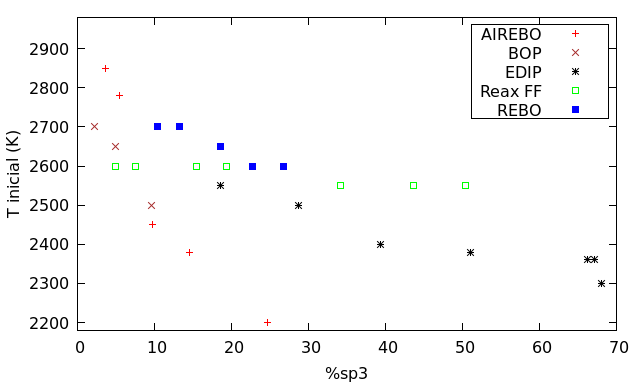
\includegraphics[width=0.5\textwidth]{datamelting.png}\\
        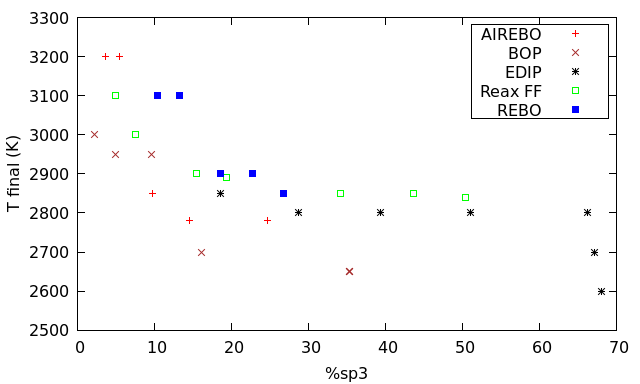
\includegraphics[width=0.5\textwidth]{datameltingfin.png}
        \caption{Initial (above) and final(below temperature of de phase change processes for Airebo-m, Bop, Edip, Reax y Rebo potentials is shown. Cycles happens in temperature windows of aprox. $200K$ and after the process the graphite structure stays until $4000K$}
        \label{fig:meltdata}
    \end{figure}
\subsection{Bulk Modulus}
Looking Bulk Moduli valued, these were obtained  making files with sample behaviour averages after an expansion and compression process in a little lenght interval compared with total bulk lenght. 

Sample average behaviour was observed in la Figure~\ref{fig:bulkproc}. In this figure it is shown a curve that can be fitted in a straight line and the Bulk Modulus can be obtained multiplying the line slope by the initial volumen. This calculation is made for AIREBO, ReaxFF, REBO y EDIP potentials. For all samples it was obtained Bulk modulus values between $100$ and $300 GPa$, that are plotted in Figure~\ref{fig:bulkdata}. 

The result are agree with Ito works {\it et al.} que presentan el Bulk Modulus para samples de aC dependiendo de la densidad de masa con values entre los 200 y 350 GPa.~\cite{RefBulk}
    \begin{figure}
        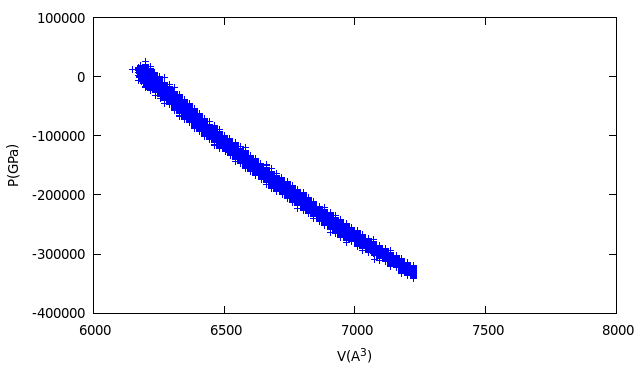
\includegraphics[width=0.5\textwidth]{bulk.png}
        \caption{Answer for one of the Bulk Modulus calculations. 2 curves sample expansion and contraction curves are shown, applying negative direction pressure. Bulk Modulus was obtained after taking the linear regression slope of a short expansion interval.}
        \label{fig:bulkproc}
    \end{figure}
    \begin{figure}
        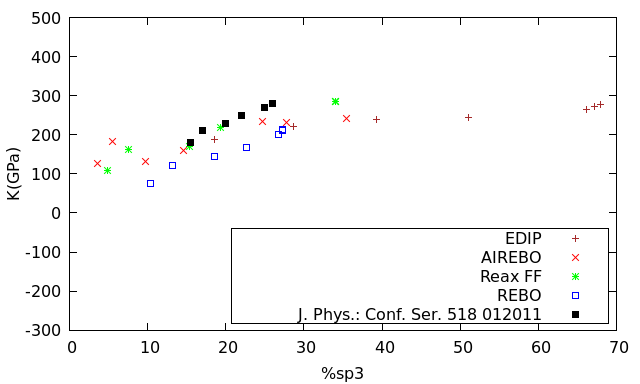
\includegraphics[width=0.5\textwidth]{databulk.png}
        \caption{Bulk Moduli for para Airebo-m, Reax, Rebo y Edip potential.  \cite{RefBulk} (that shows Bulk Moduli results for a simulation of diamond-like aC sample via DFT) is used as reference. It was observed a near result to reference for Airebo-m, REBO y EDIP potentials.}
        \label{fig:bulkdata}
    \end{figure}
\section{Conclusions}
Looking these results, it appears as a natural question: Why results are different for any potential?. Interatomic potentials were agree to different kind of matter properties. According to data observed for all used potentials, all results are agree with references, at least approximately. EDIP potential gives the nearest results. With this, it was concluded that if it wanted thermodynamic variables results nearer to data able to obtain with simulations that include quantum effects for  similar size samples (as for example DFT), a potential made of some modification to EDIP potential would be enough.

It is important to remember than in realised calculations it was worked with samples of 1000 atoms in a cubic arrange of $1.5$~nm  aprox. for every box side. This box is useful to doing low computing demand calculations, even if given statistics could not be enough. After all, to evaluate a sample where it wants to insert some defects, this is and adequated sizes  (Following NV Centers testing references \cite{NVDiamond}). 

Another observation of interest is that for the analysis part data obtained (for phase change points or for Bulk Modulus), was tagged with the starting value of sp$^3$ bond percentage for any sample. This choice has as consequence that information could not be enough to obtain an adequated relationship between sp$^3$ bond percentage and thermodynamical variables. Despite this, this work is good as a starting point.

Research made with numerical methods of aC samples is an incipient field and this development es only the begginig of a work that can grow to many directions. Possible projections for future works in the field of numerical simulations could be to put defects of similar to the ones from nanodiamonds in aC with great sp$^3$ percentage. Another one would be to measure thermodynamical and vibrational properties for this new samples (it exists ways to simulate Ramman spectroscopy in classical MD using LAMMPS and Python codes \cite{Phonopy}) and comparing this results with someones from methods like DFT, always considering times of computing at the same range that this experience.
\section{Acknowledgements}
This work was supported by Universidad Mayor Doctorate Scholarship, Fondecyt (Chilean Goverment) project \#11180557 and CEDENNA.
\bibliographystyle{cas-model2-names}
\nocite{*}
\bibliography{main}
\end{document}